\documentclass[11pt,letterpaper]{article}
\usepackage[margin=0.72in]{geometry}
\usepackage[T1]{fontenc}
\usepackage{lmodern,microtype,booktabs,graphicx,xcolor,array}
\usepackage[colorlinks=true,urlcolor=blue,linkcolor=blue]{hyperref}
\definecolor{ink}{HTML}{172B36}
\definecolor{accent}{HTML}{176B93}
\definecolor{light}{HTML}{EEF4F7}
\color{ink}
\setlength{\parindent}{0pt}
\setlength{\parskip}{6pt}
\setlength{\tabcolsep}{5pt}
\renewcommand{\arraystretch}{1.13}
\hypersetup{pdftitle={Auditing recall notification dates before building a remedy-time model},pdfauthor={James N. Jean}}
\newcommand{\CaseCount}{12}
\newcommand{\GenericCount}{6}
\newcommand{\ConflictCount}{1}
\newcommand{\UnknownCount}{5}
\newcommand{\PastCount}{7}
\newcommand{\ExpectedCount}{5}
\newcommand{\DocumentCount}{60}
\newcommand{\PageCount}{170}
\newcommand{\PlanCount}{29}
\newcommand{\FlatRows}{182}
\newcommand{\ApiRows}{113}
\newcommand{\FreezeCount}{25}
\newcommand{\FigureConditions}{190}
\newcommand{\FigureArtists}{36}
\newcommand{\ReplayOld}{3.10.11}
\newcommand{\ReplaySourcesOld}{13}
\newcommand{\ReplayNew}{3.12.14}
\newcommand{\FieldA}{2023-01-31}
\newcommand{\ApiA}{2023-03-01}
\newcommand{\FieldB}{2023-01-17}
\newcommand{\ApiB}{2023-01-17}
\newcommand{\DaysB}{0}
\newcommand{\FieldC}{2023-02-16}
\newcommand{\ApiC}{2023-03-10}
\newcommand{\FieldD}{2023-01-20}
\newcommand{\ApiD}{2023-01-20}
\newcommand{\DaysD}{0}
\newcommand{\FieldE}{2023-02-07}
\newcommand{\ApiE}{2023-03-02}
\newcommand{\DaysE}{-23}
\newcommand{\FieldF}{2023-02-09}
\newcommand{\ApiF}{2023-02-01}
\newcommand{\FieldG}{2023-03-10}
\newcommand{\ApiG}{2023-03-17}
\newcommand{\FieldH}{2023-03-17}
\newcommand{\ApiH}{2023-03-17}
\newcommand{\DaysH}{0}
\newcommand{\FieldI}{2023-02-01}
\newcommand{\ApiI}{2023-02-01}
\newcommand{\DaysI}{0}
\newcommand{\FieldJ}{2023-02-23}
\newcommand{\ApiJ}{2023-02-23}
\newcommand{\DaysJ}{0}
\newcommand{\FieldK}{2023-02-22}
\newcommand{\ApiK}{2023-02-22}
\newcommand{\DaysK}{0}
\newcommand{\FieldL}{2023-02-27}
\newcommand{\ApiL}{2023-03-15}
\begin{document}
{\Large\bfseries Auditing recall notification dates before building a remedy-time model\par}
{\large A twelve-campaign source audit and typed-event implementation exercise\par}
James N. Jean \hfill Independent research, 30 October 2026\\
{\small Source capture: 31 October 2026 UTC. Not peer reviewed. No agency endorsement.}

\section*{The practical decision}
A recall dashboard can display a notification date correctly and still supply the wrong label for a remedy-time model. Keep the event role, date precision, planned/reported state and evidence identifier together before allowing that date into an analysis.

This finite audit retains all \CaseCount{} campaigns numbered 23V001000--23V012000. Six dates match current generic notification assertions; one conflicts with a current reported date; five lack a supported past-event binding under conservative coding. No physical first-availability date is established. The deliverable is a complete case table and a local guard that rejects unsupported event conversions.

\colorbox{light}{\parbox{\dimexpr\linewidth-2\fboxsep\relax}{\textbf{Recommended action.} Use the typed notice as a notice. Investigate the conflicting source date and keep remedy availability unknown until separate evidence establishes it. A smaller or cleaner-looking label table is not evidence of a valid remedy-time target.}}

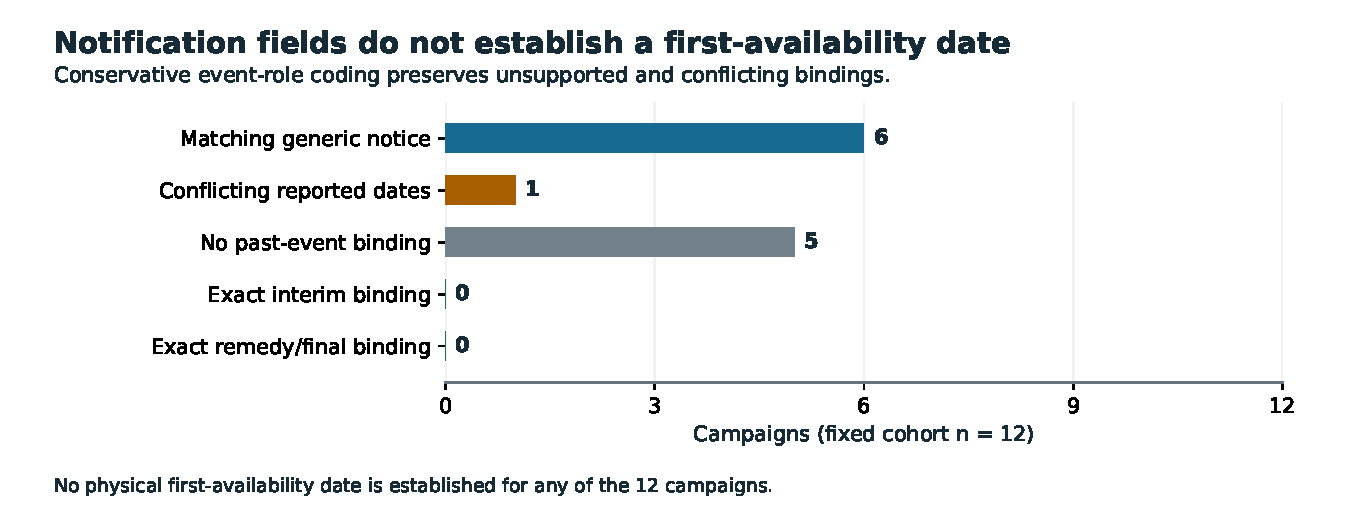
\includegraphics[width=\linewidth]{images/event_role_counts.pdf}
{\small\textbf{Figure 1.} All \CaseCount{} fixed campaigns. There are \GenericCount{} matching generic notices, \ConflictCount{} conflict and \UnknownCount{} unresolved bindings. Exact dated interim and remedy/final bindings are both zero under the coding rules. These are conservative evidence categories, not national error-rate estimates.}

\textbf{Scope.} This is descriptive source measurement and defensive software, with no fitted model, tuned threshold, prediction, repair-delivery measurement or safety validation. The original proposal to predict time to final remedy from initial Part 573 information remains unexecuted: both the outcome label and initial-vintage gates are unresolved.
\newpage

\section*{Every campaign is retained}
\small
\begin{tabular}{@{}lllllr@{}}
\toprule
Campaign & Flat ODATE & Current API date & API state & Binding & Days\\
\midrule
23V001 & \texttt{\FieldA} & \texttt{\ApiA} & expected & unresolved & n/a \\
23V002 & \texttt{\FieldB} & \texttt{\ApiB} & past & generic match & \DaysB \\
23V003 & \texttt{\FieldC} & \texttt{\ApiC} & expected & unresolved & n/a \\
23V004 & \texttt{\FieldD} & \texttt{\ApiD} & past & generic match & \DaysD \\
23V005 & \texttt{\FieldE} & \texttt{\ApiE} & past & conflict & \DaysE \\
23V006 & \texttt{\FieldF} & \texttt{\ApiF} & expected & unresolved & n/a \\
23V007 & \texttt{\FieldG} & \texttt{\ApiG} & expected & unresolved & n/a \\
23V008 & \texttt{\FieldH} & \texttt{\ApiH} & past & generic match & \DaysH \\
23V009 & \texttt{\FieldI} & \texttt{\ApiI} & past & generic match & \DaysI \\
23V010 & \texttt{\FieldJ} & \texttt{\ApiJ} & past & generic match & \DaysJ \\
23V011 & \texttt{\FieldK} & \texttt{\ApiK} & past & generic match & \DaysK \\
23V012 & \texttt{\FieldL} & \texttt{\ApiL} & expected & unresolved & n/a \\
\bottomrule
\end{tabular}
\normalsize

{\small\textbf{Table 1.} \emph{Past} means the current API explicitly says letters were mailed or notification began. \emph{Expected} remains a plan. Days is flat ODATE minus a reported API notice date, in calendar days; n/a means no comparable past assertion. A zero is source-date equality, not zero repair delay. These are current attributed assertions, not independently verified delivery.}

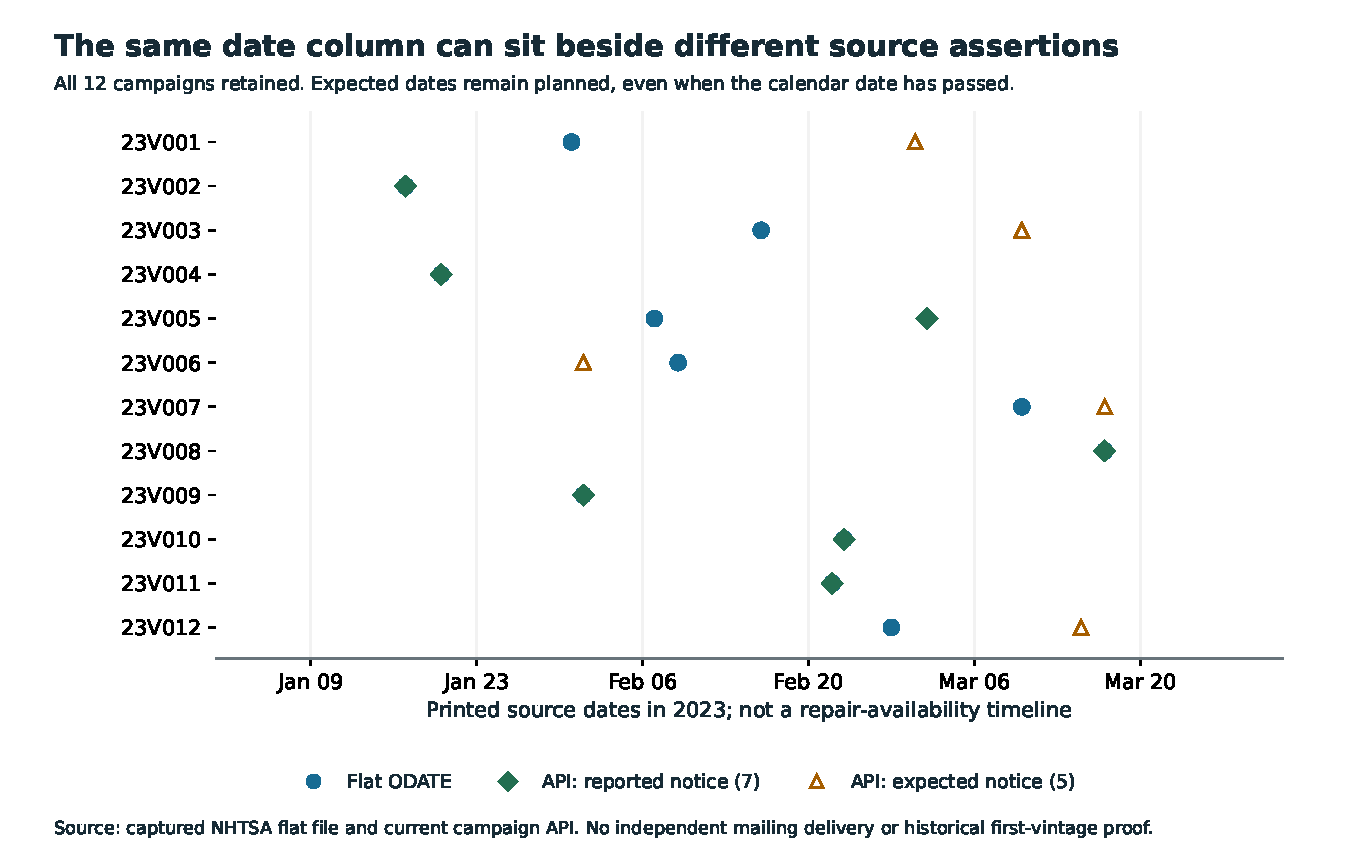
\includegraphics[width=\linewidth]{images/field_and_api_dates.pdf}
{\small\textbf{Figure 2.} The same generic flat-file date is shown beside reported or expected API assertions. Coincident markers indicate equal dates. All cases remain visible; planned dates do not become actual events just because the calendar day has passed.}

The unit is the campaign. The \FlatRows{} matching flat-file model rows and \ApiRows{} API records are different source representations; neither is an independent sample of campaigns.
\newpage

\section*{What document review changes}
\textbf{The source conflict: 23V005.} Flat ODATE is \FieldE{}, whereas the current API says owner notification letters were mailed \ApiE{}. A dated owner letter also says 2 March 2023. The signed discrepancy is \DaysE{} days. Different phases or later revisions could explain it; this audit does not determine that the agency field is erroneous. The guard holds the conflicting binding for review.

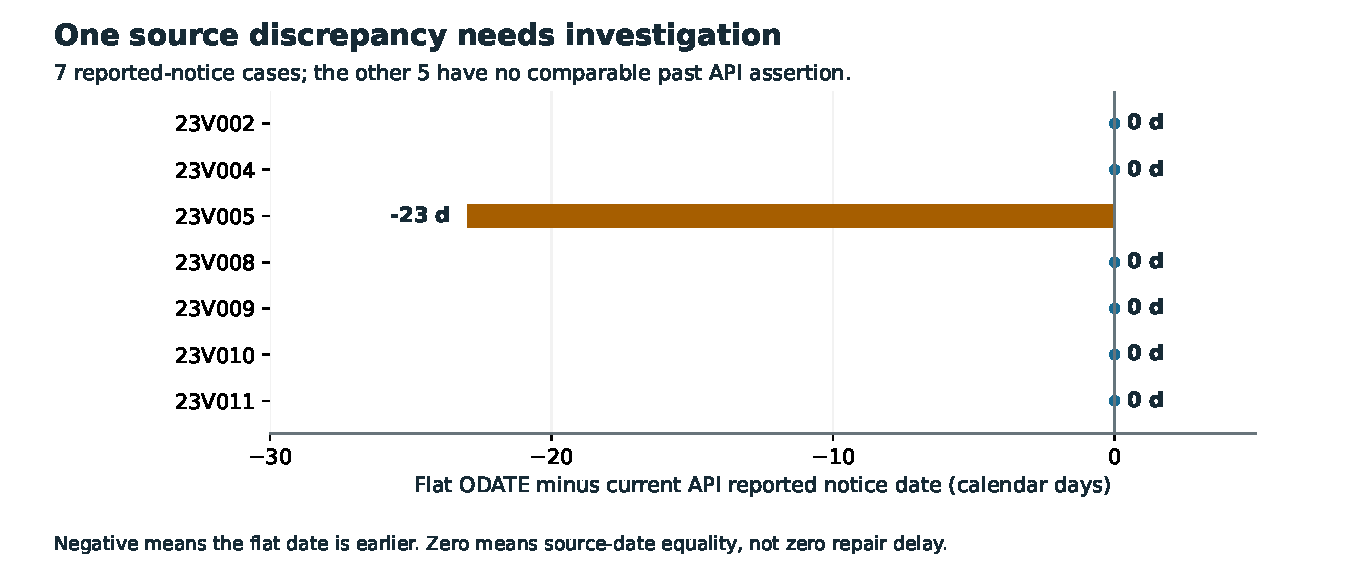
\includegraphics[width=\linewidth]{images/reported_date_differences.pdf}
{\small\textbf{Figure 3.} All \PastCount{} campaigns with a past API notification assertion. The other \ExpectedCount{} have no comparable past assertion. This is a source-date comparison, not a distribution of actual remedy delay.}

\textbf{A matching letter date is insufficient: 23V003.} Its owner letter is dated 16 February 2023, matching ODATE. The API still describes expected notification on 10 March. The printed letter day alone does not prove mailing, so the past-event binding remains unresolved. The attached service notice has a release date; that is another event role.

\textbf{Interim is not final: 23V010.} The issued interim template explicitly says the remedy is not currently available, but has no printed exact date. Later Part 573 amendments describe phased notification beginning 23 February for 2022--2023 vehicles, plus other planned model-year phases. The generic ODATE match cannot identify an exact interim or final notice, or first physical remedy availability.

\textbf{An availability assertion can still lack a day: 23V011.} The letter says \emph{Remedy is Available}, but is marked SAMPLE and dated only February 2023. The API's reported 22 February mailing remains a generic notice assertion; the sample does not establish a first-availability day.

\textbf{Channel timing matters: 23V012.} The 27 February letter says a dealer upgrade can be performed, while OTA release will not be available until mid-March. Collapsing these statements into one remedy-availability date loses their meaning.
\newpage

\section*{Sources, coding and implementation}
The campaign numbers were fixed before capture. Selection was source informed: a prior API example and one Volvo notification date were already visible. There is no blinded or representative-cohort claim.

The official campaign lists supplied 197 PDF links. A metadata filter captured 64 files. Four envelope templates were retained privately but excluded before semantic coding, leaving \DocumentCount{} eligible documents and \PageCount{} pages: \PlanCount{} templated Part 573 reports, twelve acknowledgements, eighteen owner/renotification letters and one supplemental report. Every eligible document has a public factual adjudication row with native hash, type, page, date precision, event state, short evidence and unknowns. Planned ranges, amendments, generic templates and channel-dependent statements stay distinct.

A default PDF reader reordered header columns. A source-flow extraction repair resolved all 58 structured cell comparisons between pypdf and pdfplumber. Relevant native page regions were visually inspected; not every page was visually inspected. Nine cells needed native-page visual checks because of raster content or extraction differences. One narrative date page was corrected before comparison. Earlier failed receipts are retained privately.

The code accepts an exact date and source evidence, checks campaign identity and certainty, and preserves the original event role. The six source-backed exercises produce:

\small
\begin{tabular}{@{}p{0.49\linewidth}p{0.45\linewidth}@{}}
\toprule
Input request & Outcome\\
\midrule
Reported generic notice with matching evidence & Accept; retain generic notice role\\
Same notice presented as physical availability & Reject unsupported role conversion\\
Expected notice presented as a reported event & Reject planned-as-reported input\\
Undated interim template & Reject missing exact date\\
Conflicting current notification sources & Reject ambiguous binding\\
Missing evidence identifier & Reject missing evidence\\
\bottomrule
\end{tabular}
\normalsize

The guard relies on the curated evidence table; it cannot determine that an arbitrary external assertion is true. A separately verified availability example in an authored fixture tests the interface only. No such first-availability evidence is established in this cohort.

\textbf{Validation.} Source/method hashes for \FreezeCount{} dependencies were committed before the first comparison command. Native flat/API reconciliation passed 247,156 finite conditions; retained PDF/hash/page checking passed 712 automated conditions plus the manual native-page cells. Saved-projection checks passed 720 conditions; independent SQLite joins, CASE logic, calendar arithmetic and exercise expectations passed 152. Twenty-six authored fixture tests cover invalid/ambiguous dates, leap days, conflicting roles, empty denominators and unsupported conversions. Finite passing checks do not establish universal correctness.
\newpage

\section*{Reproduce and use}
Two separate full-history checkouts, CPython \ReplayOld{} and \ReplayNew{}, reproduce all four analysis/exercise result files byte for byte, with \ReplaySourcesOld{} source projection files unchanged in each. This saved-data replay does not redownload native sources or independently repeat semantic adjudication.

\begin{verbatim}
python -m pip install -r requirements.txt
python src/replay.py --out ../recall-audit-replay
\end{verbatim}

The repository includes all twelve cases, every planned report range, the sixty-row source adjudication, the local guard, authored fixtures and the original figures. Figure checks bind \FigureArtists{} actual artists to results and verify source coordinates, numeric labels and nine asset hashes through \FigureConditions{} finite conditions. The published manuscript and figure hashes are scoped explicitly.

\textbf{Operational use.} A data engineer can use this package to review a proposed recall label table before training or reporting turnaround times. Keep the notice type and planned/reported state as separate fields. Preserve precise source identifiers and channel distinctions. Investigate a source discrepancy rather than filling it with a convenient date. This implementation is local; no production users, measured workflow savings or deployed integration are claimed.

\section*{Limits and evidence still needed}
These twelve early numbered 2023 campaigns are a finite convenience cohort, with related documents and repeated model records. Counts cannot estimate national reliability, safety performance or a remedy-time distribution. Conservative rules can leave a real event unresolved. Source equality does not verify mailing delivery, notification receipt or first repair availability.

The API and flat file are captured current sources. Amended documents do not reconstruct immutable original filings, first-byte availability or what a forecaster could have known at the time. Manufacturer statements, sample letters and planned fields remain attributed assertions. Physical first availability is unknown for all \CaseCount{} cases; it is never filled from ODATE.

A predictive follow-up needs a defensible event definition, independently documented labels and feature snapshots at the prediction origin. A prospective guard evaluation needs a monitored workflow and recorded error handling. Neither is supplied by this descriptive audit. There is no causal, clinical, safety, financial-benefit or new-estimator claim.

\section*{Primary sources and publication boundary}
{\small
NHTSA, \href{https://www.nhtsa.gov/nhtsa-datasets-and-apis}{Datasets and APIs};
\href{https://static.nhtsa.gov/odi/ffdd/rcl/RCL.txt}{recall flat-file dictionary};
\href{https://www.nhtsa.gov/recalls}{campaign search and associated documents};
\href{https://www.nhtsa.gov/about-nhtsa/terms-use}{Terms of Use}.
Exact campaign API URLs, native PDF URLs and source hashes are in the data manifests. The fixed capture and necessary factual projection are attributed; code uses MIT.

Full native archives, PDFs, contact blocks and vehicle identifiers remain private. This is an independent program manuscript, not a formal-publication submission. Azure optimization and other formal-publication projects are excluded from this repository.
}
\end{document}
